\documentclass{amsart}
\usepackage[utf8]{inputenc}
\usepackage[english]{babel}
\usepackage{amsmath}
\usepackage{tikz-cd}

\newtheorem{theorem}{Theorem}
\newtheorem{lemma}[theorem]{Lemma}
\newtheorem{statement}[theorem]{Statement}

\newcommand{\Z}{\mathbb{Z}}
\newcommand{\R}{\mathbb{R}}
\newcommand{\dprime}{{\prime\prime}}
\DeclareMathOperator{\im}{im}
\DeclareMathOperator{\interior}{int}

\setlength{\textwidth}{\paperwidth}
\addtolength{\textwidth}{-1.6in}
\setlength{\textheight}{\paperheight}
\addtolength{\textheight}{-1.8in}
\calclayout

\begin{document}
	\begin{statement}
		Let $Y \subseteq X$ be a pair of compact Hausdorff spaces such that for any $p \in Y$ and any open neighborhood $V$ of $p$ in $X$ there exists an open neighborhood $U \subset V$ of $p$ such that $\im \big(\widetilde H_\bullet(U \cap Y) \to \widetilde H_\bullet(V)\big) = 0$. Then, $\im \big(H_d(Y) \to H_d(X)\big)$ is finitely generated for every $d$.
	\end{statement}
	
	\paragraph{Terminology} A \textit{neighborhood} of a point is a set containing an open neighborhood of it.
	
	\begin{theorem}
		Let $X$ be locally compact and Hausdorff and $Y \subseteq X$ compact.
		\begin{itemize}
			\item[$(r^n)$] If $K$ and $M$ are compact subsets of $X$ with $\widetilde K = K \cap Y \subset \interior M$, then $\im r^n_{\widetilde K, M}$ is finite.
			\item[$(r^n_\bullet)$] If $V$ is an open neighborhood in $X$ of $y \in Y$ there exist another such neighborhood $U \subseteq V$ such that $\im r^n_{U \cap Y, V}$ is finite.
		\end{itemize}
		Then, $(r^{n-1})$ together with $(r^n_\bullet)$ imply $(r^n)$.
	\end{theorem}
	
	\begin{proof}
		Let $M$ be fixed and let $\sigma$ be the set of compact subsets $K$ with $K \cap Y \subseteq \interior M$ such that $K$ has a neighborhood $U_K$ such that $\im r^n_{U_K \cap Y, M}$ is finite.
		
		Recall the following fact:
		$(\ast)$ A space $S$ if locally compact and Hausdorff if and only if for every point $p$ of $S$, any neighborhood of $p$ contains a compact neighborhood of $p$.
		
		For $i \in \{1, 2\}$ consider $K_i \in \sigma$ and let $K_i^\prime$ and $K_i^\dprime$ be compact neighborhoods of $K_i$ such that
		\begin{equation*}
		K_i \subseteq K_i^\dprime \subseteq \interior K_i^\prime \subseteq K_i^\prime \subseteq U_i,
		\end{equation*}
		where $\im r^n_{U_i \cap Y, M}$ is finite. 
		We can construct such compact neighborhoods using $(\ast)$ as follows:
		
		Consider for each $p \in K_i$ a compact neighborhood $K^\prime_i(p) \subseteq U_i$ and let $K_i^\dprime(p) \subseteq \interior K_i^\prime(p)$ be another compact neighborhood of $p$. The collection of open sets $\interior K_i^\dprime(p)$ covers the compact $K_i$, and a finite union of the corresponding compact neighborhoods form the desired $K_i^\prime, K_i^\dprime$.
		
		Furthermore, we have $K^\dprime_1 \cap K^\dprime_2 \cap Y \subseteq \interior(K_1^\prime \cap K_2^\prime \cap Y)$. To see this (if not immediately), take $p \in K^\dprime_1 \cap K^\dprime_2 \cap Y$, since by assumption there exist open sets $V_i$ in $X$ such that $p \in V_i \cap K_i^\prime$. Letting $V = V_1 \cap V_2$ we have $p \in V \cap (K^\prime_1 \cap K^\prime_2)$ and, since $p \in Y$, $p \in V \cap (K^\prime_1 \cap K^\prime_2 \cap Y)$ implying the claim.
		
		Using $\widetilde{K}$ to denote $K \cap Y$ we have the commutative diagram
		\begin{equation*}
		\begin{tikzcd}
		& \arrow[r] \arrow[d] H^n(M) & H^n(M) \oplus H^n(M) \arrow[d] \\
		H^{n-1}(\widetilde K_1^\prime \cap \widetilde K_2^\prime) \arrow[r] \arrow[d] & 
		H^{n}(\widetilde K_1^\prime \cup \widetilde K_2^\prime) \arrow[r] \arrow[d] &
		H^{n}(\widetilde K_1^\prime) \oplus H^n(\widetilde K_2^\prime) \\
		H^{n-1}(\widetilde K_1^\dprime \cap \widetilde K_2^\dprime) \arrow[r] & 
		H^{n}(\widetilde K_1^\dprime \cup \widetilde K_2^\dprime). &
		\end{tikzcd}
		\end{equation*}
		The upper right square has finite image because $\im r^n_{\widetilde K^\prime_i, M}$ is finite. The bottom left square has a finite image using property $(r^{n-1})$. From standard homological algebra using that the middle row is exact we conclude that $K_1 \cup K_2 \in \sigma$.
		
		Notice that because of $(r_\bullet^n)$ and $(\ast)$, the collection $\sigma$ contains a compact neighborhood of each $y \in Y$.
		
		Let $K$ compact such that $\widetilde K = K \cap Y \subset \interior M$. We can cover $\widetilde{K}$ with finitely many sets in $\sigma$ and conclude that $K$ is itself in $\sigma$.
	\end{proof}
\end{document}

\begin{lemma}
	Let $Y \subseteq X$ be a pair of compact Hausdorff spaces, then $(r^0)$ above holds. 
\end{lemma}

\begin{proof}
	Let $K$ and $M$ be compact subsets of $X$ with $\widetilde K = K \cap Y \subset \interior M$. For every $y \in \widetilde K$, considering the open neighborhood $\interior M$, let $U_y$ be the open set such that $\im r_{U_y \cap Y, M}$ is finite. Cover $\widetilde K$ with a finite number of such open sets $\{v_1, \dots v_n\}$. Since
	\begin{equation*}
	\begin{tikzcd}
	\bigoplus_i^n H_0(\widetilde{U_i}) \arrow[r] \arrow[d, "0"] & H_0(\widetilde{K}) \arrow[d] \arrow[r] & 0 \\
	\bigoplus_i^n H_0(M) \arrow[r] & H_0(M) &
	\end{tikzcd}
	\end{equation*}
	commutes, we have the desired conclusion.
	(Verify the universal coefficients theorem here recalling that $H_0$ is always free.)
\end{proof}

\paragraph{NOT \textit{Counterexample}} Let $Z = \left\{\left(0, 2^{-n}\right)\ |\ n \geq 0\right\} \cup \{(0, 0)\} \subset \R^2$. Let $X$ be a model of the suspension of $Z$ embedded in $\R^2$. The space $X$ is path-connected, Hausdorff, compact, and with infinite first homology. Furthermore, locally $H_1 = 0$. Taking $Y = X$ gives a counterexample.

\begin{equation*}
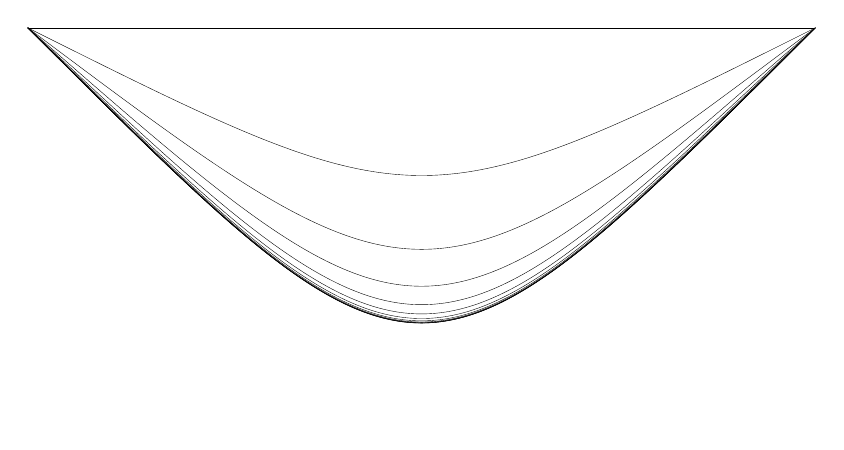
\begin{tikzpicture}[scale=5]
\foreach \i in {0,1,2,...,12}{
	\draw[line width=0.05mm] (-1,1) .. controls (0,1/2^\i) .. (1,1);
}
\end{tikzpicture}
\end{equation*}

A diagram to keep in mind
\begin{equation}
\begin{tikzcd}
\Z^{\infty} \arrow[r, "0"] & \Z^{\infty} \arrow[r, "1"] & \Z^{\infty} \arrow[r, "0"] & \Z^{\infty} \arrow[r, "1"] & \Z^{\infty} \\
\Z^{\infty} \arrow[r, "1"] \arrow[u, "0"] & \Z^{\infty} \arrow[r, "0"] \arrow[u, "0"] & \Z^{\infty} \arrow[r, "1"] \arrow[u, "1"] & \Z^{\infty} \arrow[r, "0"] \arrow[u, "0"] & \Z^{\infty} \arrow[u, "0"]
\end{tikzcd}
\end{equation}

Consider the following general diagram
\begin{equation}
\begin{tikzcd}
A_1 \arrow[r, "s_1"] & A_2 \arrow[r, "s_2"] & B \arrow[r, "t_1"] & C_1 \arrow[r, "t_2"] & C_2 \\
X_1 \arrow[r, "g_1"] \arrow[u, "0"] & X_2 \arrow[r, "g_2"] \arrow[u, "0"] & Y \arrow[r, "h_1"] \arrow[u, "f"] & Z_1 \arrow[r, "h_2"] \arrow[u, "0"] & Z_2 \arrow[u, "0"]
\end{tikzcd}
\end{equation}
